\section{Background}
In this section we will discuss the various tools and break down how we will
formulate the project. In the next section we will discuss our proposition of
how to achieve these goals.

\subsection{Q-Learning}
For this project we will be using a Q-Learning algorithm to play these
videogames. The Q-Learning algorithm is a simple reinforcement learner that
follows Bellman's Equation. A Q matrix can be defined where each row represents
a different state and each column represents an action for that state. These
can be used to solve different Markov Decision Processes (MDPs). An example
MDP is shown in Figure~\ref{fig:MDP}.

\begin{figure}[ht]
    \centering
    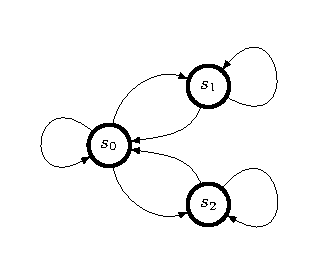
\includegraphics[width=0.6\textwidth]{MDP.pdf}
\caption{Sample Markov Decision Process}
    \label{fig:MDP}
\end{figure}
Each node, labeled $s_i$, represents a state and the connections between nodes
represent actions. Each action has an associated probability with it. There 
are certain ``rewards" that an actor gets for taking certain actions, $a$, which
leaves them in a new state, $s'$. We then want to find a set of actions, also
known as a policy ($\pi$) that gives us our maximal value ($V$). Knowing this
we want to create a learner that will learn the best policy, set of actions,
that will maximize its reward. The Bellman Equation, Equation~\ref{eq:Bell}, 
does just this. In this equation $\alpha$ represents the learning rate, 
$\gamma$ is the discount rate, and $Q(s',a')$ is the value in our $Q$ matrix
given the next state and action.
\begin{equation}
    Q(s,a) = Q(s,a) + \alpha(r + \gamma \max_{a'}Q(s',a') - Q(s,a))
    \label{eq:Bell}
\end{equation}
Essentially what we are doing is looking at the reward we get for taking an 
action and all future rewards given our best policy. A discount rate is 
applied so that rewards that are achieved sooner are weighted more heavily
than rewards further away. A simple example of why we might want to do this
is because if we give a mouse a reward for completing a maze we want the mouse
to finish the maze as fast as possible and not take an infinite time to finish.
The learning rate applies a weight to to our new reward and future rewards. 
Additionally all actions are probabilistic. If we have the actions forward,
left, and right, if we select forward there is still a probability that the
agent goes left or right. This is commonly known as a Monte-Carlo walk (or
Drunken Walk). 

For our videogames we discussed that there are potentially an unknown number
of states. There are also limitations in computational hardware. To account
for this we can simply limit the depth of our lookahead values. This will
create an approximate Q-Learner and allow us to solve problems with unknown
or infinite number of states. 

\subsection{Deep Q-Learning}
An extension of Q-Learning is deep Q-Learning (DQN) is by using a neural network 
to compute the above solution. We can accomplish this because a neural network 
is a universal function approximater, meaning it can approximate any function. 
Following DeepMind's work~\cite{DeepMind}, if we rewrite the Bellman Equation as
\begin{equation}
    Q^*(s,a) = \mathbb{E}_{s'\sim\mathcal{E}}\left[r + \gamma\max_{a'}Q^*(s',a')\right]
\end{equation}
We can generate a loss function $L_i(\theta_i)$
\begin{equation}
    L_i(\theta_i) = \mathbb{E}_{s,a\sim\rho(\dot)}\left[(y_i - Q(s,a;\theta_i))^2\right]
\end{equation}
where $y_i = \mathbb{E}_{s'\sim\mathcal{E}}\left[r + \gamma\max_{a'}Q(s',a';\theta_{i-1})\right]$. Recognizing that this is the same format as the Mean Square
Error (MSE) we can generate the following gradient (Equation~\ref{eq:DQNgrad}).

\begin{equation}
    \nabla_{\theta_i}L_i(\theta_i) = 
\mathbb{E}_{s,a\sim\rho(\dot);s'\sim\mathcal{E}}
\left[\left(r + \gamma\max_{a'}Q(s',a';\theta_{i-1}) - Q(s,a;\theta_i)\right) 
\nabla_{\theta_i}Q(s,a;\theta_i)\right]
\label{eq:DQNgrad}
\end{equation}

Here we have everything we need to create a DQN. The property of universal 
approximation handles the lookahead depth for us. This is because a
neural network iterates to create an approximate function. Being that our
games are NP- or PSPACE-Hard this is reasonable.

\subsection{Integration into Retro}
Unfortunately SMK was not able to be integrated into Retro's environment, but
much about the environment and integration was learned along the way.
Retro relies on different ``states", which can be defined as different 
starting states. 
This is placed in quotes because the state will continuously be changing as
the agent progresses through the level, more on this later. For
this project we started with the scenario where there is a single agent
playing the 50cc Mushroom Cup. Essentially we set a place in the game where we
want our agent to start. Retro provides a UI where we can interactively play
the game and save specific states. For this example our initial state looks like
this:
\begin{figure}[h!]
    \centering
    %\includegraphics[clip,trim=0 500 0 10,width=0.55\textwidth]{1P_GrandPrix_50cc_MushroomCup.png}
    \includegraphics[width=0.55\textwidth]{1P_GrandPrix_50cc_MushroomCup.png}
    \caption{Initial state for 1P\_GrandPrix\_50cc\_MushroomCup.state}
\end{figure}
\FloatBarrier
From this we can see that in the upper half we see our player and the world
around us. In the bottom half we see the entire map and can actually identify 
certain features like coins and items. We will be focusing on the top half.

Now that we have where we want to start, we need to define everything else.  
Retro uses json files to define many different parts to the game. There are 
two important files for each game: data.json and scenario.json. Data defines
information about the level, lives, and score. Scenario defines the
ending condition and the reward structure. An example of values are shown
below
\\
\begin{figure}[h!]
\begin{minipage}{0.47\textwidth}
    \begin{lstlisting}[caption=data.json, frame=tlrb]{Name}
{
"info": {
    "lap": {
        "address": 8261825,
        "type": "|u1"
    },
    "lapsize": {
        "address": 8257864,
        "type": "|u1"
    },
    "coins": {
        "address": 8261120,
        "type": "|u1"
    },
    "minute": {
        "address": 8257796,
        "type": "|u1"
    },
    "second": {
        "address": 8257794,
        "type": |u1"
    \end{lstlisting}
\end{minipage}\hfill
\begin{minipage}{0.47\textwidth}
    \begin{lstlisting}[caption=scenario.json, frame=tlrb]{Name}
{
"done": {
    "variables": {
        "finish": {
            "reference": "coins",
            "op": "eq"
        }
    }
},
"reward": {
    "variables": {
        "rank": {
            "reward": 1.0
        }
    }
},
"actions": [
    [[], ["UP"], ["DOWN"]],
    [[], ["LEFT"], ["RIGHT"]],
    [[], ["A"], ["B"], ...
}
    \end{lstlisting}
\end{minipage}
    \caption{Snippets from data.json and scenario.json for SNES Super Mario Kart}
\end{figure}
The data.json file contains hex addresses that represent the RAM address that the
game uses to determine certain aspects of the game. We also need to add these
to a rambase value that is given by retro (warning: this is not noted within
the documentation but is required).
Additionally, scenario.json can contain information about the action set. We can
either restrict our action set to a specific set of buttons, and button 
combinations, or we can expose all possible set of actions to the agent. Initially
we will be limiting our agent, since certain actions like ["DOWN","UP"] are
not likely to be useful, excluding glitches. Super Mario Kart has the following
set of actions: Steering with the D-Pad, B for Accelerate, A to use an item, 
Y for Brakes, X for the rear-view, L or R for Hop/Power-side (same action), 
Start to pause the game, and select for Rear-View. We will limit the agent
so that it may not look behind itself, cannot pause the game, and we will select
R for hop/power-slide (because that is what I use when playing). So our new full
action set for the steering will be \{\{UP\},\{DOWN\},\{LEFT\},\{RIGHT\},
\{UP,LEFT\}, \{UP, RIGHT\}, \{DOWN,RIGHT\}, \{DOWN,LEFT\}\}. 
This represents the left side of the controller. For the right side of the 
controller we will assume that the agent can play like a human does 
(this will also limit glitches that the agent might be able to exploit). 
The controls action set will be defined as \{\{B\},\{A\},\{Y\},
\{R\},\{A,B\},\{B,R\},\{A,R\}\}. The full action set is the combination of 
actions from the steering set and the control set. 

RAM addresses can be found by using emulator tools, such as BizHawk~\cite{BH}, 
that allow for hex searching and manipulation. Some values are easy to find 
since their values in RAM identically match the values displayed on the screen.
Other values may be more difficult to find given that they may be manipulated
by the program. An example of finding a memory address in BizHawk is shown in
Figure~\ref{fig:hex} in the Appendix. We were unable to find all the required
address on our own, but a prominant Speed-Runner\footnote{People who compete
to finish a game as quickly as possible} named SethBling~\cite{SethBling} 
kindly provided me with Lua scripts to help me find the missing addresses.
Section~\ref{sec:RAM} provides a more detailed discussion on finding RAM values.

To summarize the integration: we need to fully define how our agent will receive
rewards, when the agent ends, and our action set.

\subsection{Rewards}
Defining rewards is always a challenging problem in any machine learning task. 
There are many fantastic examples where a well thought out reward function leads
to outcomes not expected by the machine learning engineer. Rewards can be 
simple or extremely complex. For example a simple reward function for Super
Mario Bros might be to use the x position on the screen and reward the agent
for making forward progression through the level. 

A more detailed discussion of rewards for Super Mario Kart are given in the
appendix~\ref{sec:SMKRewards}. Additionally sections are provided for 
determining the end state~\ref{sec:endstate} and visualizing the environment
\ref{sec:env} specifically in the SMK world.

